\documentclass{article}
\usepackage{amsmath} % Нужно для элементов математики.
\usepackage[utf8]{inputenc}
\pagestyle{empty}

\usepackage[usenames,dvipsnames,svgnames,table]{xcolor}
\usepackage{tikz-timing}[2009/05/15]
\usepackage{multicol}
\usepackage[T2A]{fontenc}
\usepackage[russian]{babel}
\usepackage[left=2.5cm, right=1.5cm, vmargin=2.5cm]{geometry}
\setlength\parindent{0pt} % Удалить отступы из параграфов.

\usepackage{listings} %% собственно, это и есть пакет listing.
\usepackage{caption}
\DeclareCaptionFont{white}{\color{white}} % это сделает текст заголовка.
\DeclareCaptionFormat{listing}{\colorbox{gray}{\parbox{\textwidth}{#1#2#3}}}
\captionsetup[lstlisting]{format=listing,labelfont=white,textfont=white}
\renewcommand\labelenumi{\theenumi)}



\begin{document}
	\lstset{ %
		language=java,                 % выбор языка для подсветки (здесь это java).
		basicstyle=\small\sffamily, % размер и начертание шрифта для подсветки кода.
		numbers=left,               % где поставить нумерацию строк (слева\справа).
		numberstyle=\tiny,           % размер шрифта для номеров строк.
		stepnumber=1,                   % размер шага между двумя номерами строк.
		firstnumber=1,
		numberfirstline=true
		numbersep=5pt,                % как далеко отстоят номера строк от подсвечиваемого кода.
		backgroundcolor=\color{white}, % цвет фона подсветки - используем \usepackage{color}.
		showspaces=false,            % показывать или нет пробелы специальными отступами.
		showstringspaces=false,      % показывать или нет пробелы в строках.
		showtabs=false,             % показывать или нет табуляцию в строках.
		frame=single,              % рисовать рамку вокруг кода.
		tabsize=2,                 % размер табуляции по умолчанию равен 2 пробелам.
		captionpos=t,              % позиция заголовка вверху [t] или внизу [b].
		breaklines=true,           % автоматически переносить строки (да\нет).
		breakatwhitespace=false, % переносить строки только если есть пробел.
		escapeinside={\%*}{*)}   % если нужно добавить комментарии в коде.
	}

	\begin{titlepage}


		\center % Сделать все по-центру.

		%----------------------------------------------------------------------------------------
		%	Верхний колонтитул.
		%----------------------------------------------------------------------------------------

		ФЕДЕРАЛЬНОЕ ГОСУДАРСТВЕННОЕ АВТОНОМНОЕ ОБРАЗОВАТЕЛЬНОЕ УЧРЕЖДЕНИЕ ВЫСШЕГО ОБРАЗОВАНИЯ\linebreak
		«Санкт-Петербургский политехнический университет Петра Великого»\\[2cm] % Название университета.
		\textsc{\Large Институт компьютерных наук и технологий}\\[6.5cm] % Название кафедры.

		%----------------------------------------------------------------------------------------
		%	Заголовок.
		%----------------------------------------------------------------------------------------

		{ \huge \bfseries Курсовая работа	\\
			\Large \mdseries “Реализация Системы Массового Обслуживания”}\\[6.5cm] % Заголовок документа.

		%----------------------------------------------------------------------------------------
		%	Автор.
		%----------------------------------------------------------------------------------------
		\begin{multicols}{2}
			\begin{flushright} \large

				{Выполнил студент группы: 3530904/00104:}\\[0.5cm]

				{Преподаватель:\\}

			\end{flushright}
			\begin{flushright}

				{Почернин В. С.}\\[0.5cm] % Мое имя.


				Смирнов Н. Г. % Имя преподавателя.

			\end{flushright}
		\end{multicols}

		%----------------------------------------------------------------------------------------
		%	Дата.
		%----------------------------------------------------------------------------------------
		\flushright{
			{\today}\\[0.5cm]
		}
		\centering{
			Санкт-Петербург\\
			2022
		}

		\vfill % Заполнить остаток страницы пустым местом.

	\end{titlepage}


	\tableofcontents
	\newpage

	\section{Первый этап}


	\subsection{Бланк задания с заполненными исходными данными к работе}

	\subsubsection{Вариант задания}
	ИБ-ИЗ2-ПЗ1-Д10З1-Д10О3-Д2П2-Д2Б2-ОР1-ОД1

	\subsubsection{Источники}
	\begin{itemize}
		\item ИБ - бесконечный источник.
		\item ИЗ2 - равномерный закон распределения.
	\end{itemize}

	\subsubsection{Приборы}
	\begin{itemize}
		\item ПЗ1 - экспоненциальный закон распределения времени обслуживания.
	\end{itemize}

	\subsubsection{Описание дисциплин постановки и выбора}
	\begin{itemize}
		\item Д10З1 - относительный приоритет на обслуживание - запись в буфер, если есть место по кольцу.
		\item Д1003 - дисциплина отказа - самая старая в буфере.
	\end{itemize}

	\subsubsection{Дисциплины постановки на обслуживание}
	\begin{itemize}
		\item Д2Б2 - принцип выбора заявки из буфера LIFO.
		\item Д2П2 - выбор прибора по кольцу.
	\end{itemize}

	\subsubsection{Виды отображения результатов работы программной модели}
	\begin{itemize}
		\item ОД1 - отображение динамики функционирования модели: календарь событий, буфер и текущее состояние.
		\item ОР1 - отображение результатов: сводная таблица результатов.
	\end{itemize}


	\subsection{Формализованная схема ВС}
	Для освоения функционирования СМО, рассмотрим формализованную схему её работы:
	\begin{figure}[!htbp]
	\centering
	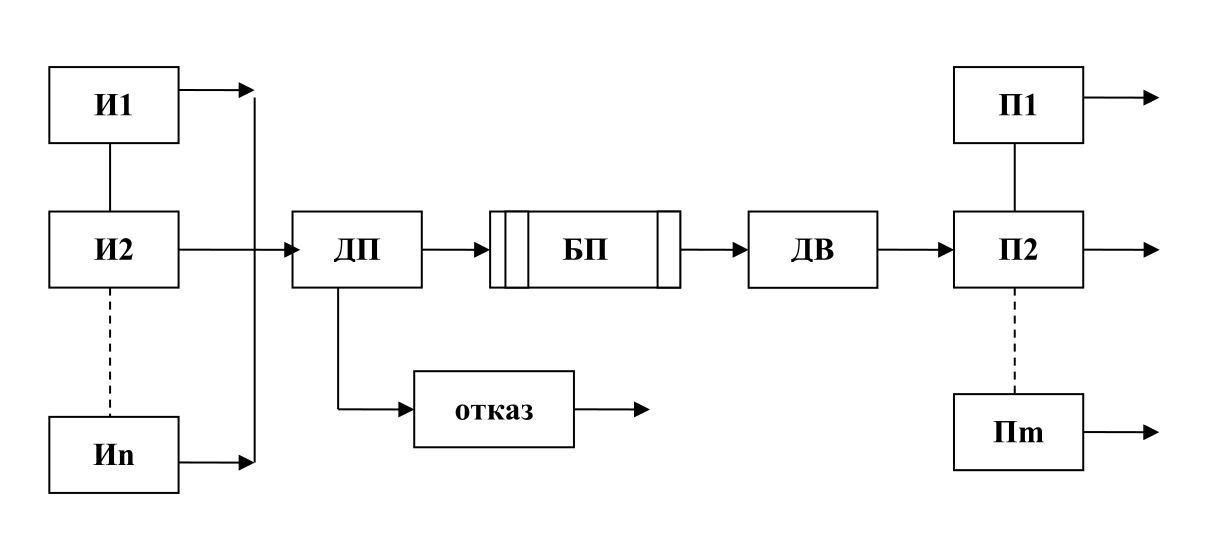
\includegraphics[width=15cm,height=\textheight,keepaspectratio]{smo.png}\\
	\caption{Формализованная схема ВС}
	\end{figure}

	\begin{itemize}
		\item Иi ($i=1..n$) представляют собой источники заявок, которые генерируют заявки. Все n источников вместе образуют входной поток заявок.
		\item Заявки, сгенерированные в источниках попадают на ДП - диспетчер постановки заявок в очередь. Он организует отказ или выбивание заявки из БП, если в буфере не осталось свободных мест, либо же отправляет заявку на обслуживание или в буферную память в случае отсутствия свободных приборов.
		\item БП - буферная память (место для хранения очереди заявок),  в которой хранятся заявки от различных источников.
		\item ДВ - диспетчер выбора заявок из очереди отправляет заявку из буфера на свободный прибор.
		\item П - приборы, которые обслуживают заявки и создают тем самым выходной поток заявок после обслуживания.
	\end{itemize}

	На основе этого, мы можем проследить путь заявки, вошедшей в модель системы:
	\begin{enumerate}
		\item Постановка заявки в буфер.
		\item Отказ или выбивание (удаление) заявки из переполненного буфера.
		\item Выбор заявки из БП на обслуживание.
		\item Поиск свободного прибора.
		\item Обслуживание заявки прибором.
		\item Выход заявки из СМО.
	\end{enumerate}
	При этом, вся логика прохождения заявок по системе определяется диспетчерами ДП и ДВ, когда источники и приборы их только генерируют и обслуживают соответственно.


	\subsection{Временная диаграмма своего варианта}
	\section{Временная диаграмма функционирования системы}
	Рассмотрим временную диаграмму функционирования системы, на которой покажем
	\begin{itemize}
		\item Моменты постановки заявок на приборы.
		\item Заполнение буферной памяти по заданной дисциплине постановки заявки в буфер.
		\item Отказ заявке или выбивание её при отсутствии свободных мест в БП.
		\item Функционирование дисциплины выбора заявок из буфера и дисциплины выбора приборов.
	\end{itemize}
	Пусть наша система будет состоять из 3 источников (И1, И2, И3), 2 позиций в буфере (Б1, Б2) и 2 приборов (П1, П2). Получим следующую диаграмму:

	\begin{tikztimingtable}
		И1 				& L G L L L L L L L L L L G L L L L L L L L L L L L L L L L L L L\\
		И2 				& L L L G L L L L L L G L L L L G L L L L L L L L L L L L L L L L L\\
		И3 				& L L L L L G L L G L L L L L L L L L L L L L L L L L L L L L L L\\
		П1 				& L 14D{1} 15D{2}\\
		П2 				& L L L 12D{2} L L 13D{1}\\
		П3 				& L L L L L 10D{3} L L L L 11D{2}\\
		Б1 				& L G L L L L L L G L L L L L L G L L G L L L L L L L L L L L L L L L\\
		Б2 				& L L L G L L L L L L G L L L L L L L L L L G L L L L L L L L L L L\\
		Б3 				& L L L L L G L L L L L L G L L L L L L G L L L L L L L L L L L L L\\
		\\
		Постановка      & L G L L G L L G L L G L L G L L G L L G L L L L L L L L L L L L L L L L L\\
		Изъятие         & L G L L G L L G L L L L L L L L L L G L L G L L G L L L L L L L L L L L\\
		\extracode
		\tablerules
		\begin{pgfonlayer}{background}
		\end{pgfonlayer}
	\end{tikztimingtable}

	\begin{itemize}
		\item Вначале мы видим, как 3 заявки поочереди создаются на источниках с первого по третий и, проходя через буфер (заходя туда по кольцу), моментально оказываются на приборах (куда они также попадают по кольцу).
		\item Затем, опять по правилу кольца, заявки с источников 3, 2 и 1 попадают на буферы 1, 2 и 3, в то время, как первые 3 заявки продолжают обрабатываться приборами, следовательно, у нас происходит заполнение буферной памяти.
		\item Внезапно, источник И2 генерирует еще одну заявку, но в буфере уже заполнены места, поэтому, приходится применять дисциплину отказа - самая старая в буфере. Заявка в буфере Б1 от источника И3, являясь самой старой, выбивается из буфера новоиспеченной заявкой от И2.
		\item Далее, по стечению обстоятельств, все три прибора одновременно заканчивают работу над своими заявками, благодаря чему мы можем увидеть работу дисциплин выбора заявок из буфера и выбора приборов. Так, как мы имеем выбор из буфера LIFO, сначала пойдет заявка с Б1, затем с Б3 и только потом Б2. Приборы же, продолжая выбираться по кольцу, возьмут заявки в порядке П1, П2, П3, так как последним прибором, взявшим заявку был П3.
	\end{itemize}

	\newpage

	\subsection{Краткие ответы на контрольные вопросы задания}

	\begin{enumerate}
		\item Назовите типы источников, опишите принципы их работы, различия между ними.

		\textbf{Ответ:} Источники бывают двух типов: бесконечные и конечные.

		Бесконечные источники генерируют заявка, после чего определяют (по определенному закону) интервал для генерации следующей заявки. Заявка попадает в систему в момент генерации и проходит по ней свой индивидуальный путь.

		В конечных источниках в определенный момент генерируется и отправляется в систему пакет заявок (из конечного числа заявок). Каждая заявка проходит свой индивидуальный путь по системе. Следующий пакет от такого источника генерируется тогда, когда последняя заявка из предыдущего пакета удаляется из системы (в результате обслуживания или отказа). Момент генерации определяется случайным интервалом между пакетами и новый пакет состоит из того же количества заявок.
		\item Можно ли сказать, что бесконечный источник есть частный случай конечного?

		\textbf{Ответ:} Как мне кажется, мы не можем назвать бесконечный источник частным случаем конечного. Действительно, мы можем считать одну заявку пакетом размера 1, однако случае конечного источника мы имеем четкое условие: "Момент генерации следующего пакета определяется событием, когда последняя заявка этого пакета удаляется из системы". В случае эе бесконечного источника следующая заявка может сгенерироваться в любой момент времени, в том числе тогда, когда предыдущая заявка еще находится в системе.
		\item Опишите два принципа построения моделирующего алгоритма, их преимущества и недостатки.

		\textbf{Ответ:} Существуют два подхода к построению моделирующего алгоритма ВС: подход Дельта-Т и подход особых событий.

		Подход Дельта-Т является универсальным методом построения моделирующего алгоритма, в котором состояние объекта проверяется через фиксированный интервал времени. Каждый момент времени $t_i=t_{i-1}+\Delta{t_{i-1}}$ мы получаем приближенные значения характеристик исследуемого объекта. Сам промежуток $\Delta{t}$ должен быть настолько мал, чтобы не пропустить событие в моделирующей системе, которое должно быть учтено при выбранной детальности моделирования. Метод удобен тем, что он является универсальным, однако, есть и недостаток: при его использовании постоянно проверяется состояние объектов моделирования, не изменяющихся при особо малых $\Delta{t}$, что делает метод неэффективным.

		Подход особых событий мы руководствуемся тем, что интервалы времени, в которых состояние не меняется не представляют для нас интереса. Только значимые (изменяющие состояние) переходы системы имеют для нас значение. Они определяются особыми состояниями или событиями, например:
		\begin{itemize}
			\item Поступление заявки в СМО (момент генерации заявки источником).
			\item Освобождение прибора (готовность прибора взять заявку на обслуживание).
			\item Окончание процесса моделирование, т. е. момент прекращения генерации заявок источниками.
		\end{itemize}
		Достоинством является эффективность данного принципа, из-за чего именно он используется в настоящей работе. К недостаткам же можно отнести сопутствующую сложность отслеживания вышеприведенных событий.
		\item Опишите дисциплины буферизации и постановки заявки на обслуживание, заданные в вашем варианте.

		\textbf{Ответ:} в моем варианте дисциплинами буферизации являются Д10З1 - запись в буфер, если есть место по кольцу и Д1003 - дисциплина отказа - самая старая в буфере. Дисциплинами постановки заявки на обслуживание являются Д2Б2 - принцип выбора заявки из буфера LIFO и Д2П2 - выбор прибора по кольцу. Рассмотрим каждую из них.

		\begin{itemize}
		\item Д1031 - запись в буфер, если есть место по кольцу. При такой дисциплине поиск свободного места в буфере осуществляется, начиная с номера места, следующего за последним занятым. В случае, если указатель, который ищет свободное места его не найдет - начнет действовать дисциплина, организующая отказ или выбивание заявки из БП.
		\item Д1003 - дисциплина отказа - самая старая в буфере. Эта дисциплина рассматривает только время прихода заявок в систему (момент генерации заявок источником). Заявка, раньше других вставшая в буфер получает отказ, уходит из системы и на её место встает пришедшая заявка.
		\item Д2Б2 - принцип выбора заявки из буфера LIFO (последним пришел - первым обслужен). В этом лсучае раньше других будет выбрана из буфера та заявка, которая пришла последней.
		\item Д2П2 - выбор прибора по кольцу. Поиск свободных приборов здесь каждый раз начинается с указателя и заявка встает на обслуживание в первый из найденных приборов.
		\end{itemize}
		\item Назовите некоторые варианты (комбинации) значений входных параметров, при которых на представленной временной диаграмме могут появиться отказы из БП и будут хорошо проиллюстрированы дисциплины выбора приборов и выбора заявок.

		\textbf{Ответ:} отказы из БП могут появиться тогда и только тогда, когда любой из источников генерирует заявку в то время, как буфер находится в заполненном состоянии. Например, мы получили 6 заявок от источников, 3 отправились на приборы, 3 в буфер (который после этого заполнился). Генерируется 7-я заявка, которой нет места в буфере, из-за чего применяется дисциплина отказа.

		Выбор заявок можно явно увидеть, если, например, заполнить по очереди весь буфер и заметить, что забираться заявка будет в обратном порядке. Это покажет нам, что буфер работает как стек, то есть по правилу LIFO.

		Что касается приборов, мы можем заметить их выбор по кольцу в самом начале, когда они начнут по очереди заполняться заявками. Если же затем приборы одновременно закончат обрабатывать заявки, то новыми заявками они начнут заполняться в том же порядке, поскольку указатель кольца начнет с первого прибора (так как последним прибором был последний прибор в кольце).
	\end{enumerate}


\end{document}